\documentclass{beamer}
\usepackage{graphicx}
\usepackage{amsmath}
\usepackage{amsfonts}
\usepackage{amssymb}
\usepackage{listings}
\usepackage{tikz}
\definecolor{mygray}{rgb}{0.92,0.92,0.92}
\usetheme{Montpellier}
\usecolortheme{beaver}

\begin{document}

\section{Group Meeting}
\title{Group Meeting \\ Week 4, Spring 2019}
\author{Brandon Gusto} %
\institute{Dept. of Scientific Computing \\ Florida State University}
\date{\today}
\frame{\titlepage}

\section{Multiresolution Scheme}

\begin{frame}{Hybrid Wavelet/AMR Scheme}
    \begin{columns}
        \begin{column}{0.58\textwidth}
            The goal of this project is to marry the benefits of wavelet analysis with the more developed AMR strategies:
            \begin{itemize}
                \item can wavelet sensors augment LTE for refinement?
                \item can regularity information reduce computational expense on fine grids?
            \end{itemize}
        \end{column}
        \begin{column}{0.44\textwidth}
            \scalebox{0.4}{
                % GNUPLOT: LaTeX picture
\setlength{\unitlength}{0.240900pt}
\ifx\plotpoint\undefined\newsavebox{\plotpoint}\fi
\sbox{\plotpoint}{\rule[-0.200pt]{0.400pt}{0.400pt}}%
\begin{picture}(1500,900)(0,0)
\sbox{\plotpoint}{\rule[-0.200pt]{0.400pt}{0.400pt}}%
\put(171.0,131.0){\rule[-0.200pt]{4.818pt}{0.400pt}}
\put(151,131){\makebox(0,0)[r]{$-0.5$}}
\put(1419.0,131.0){\rule[-0.200pt]{4.818pt}{0.400pt}}
\put(171.0,277.0){\rule[-0.200pt]{4.818pt}{0.400pt}}
\put(151,277){\makebox(0,0)[r]{$0$}}
\put(1419.0,277.0){\rule[-0.200pt]{4.818pt}{0.400pt}}
\put(171.0,422.0){\rule[-0.200pt]{4.818pt}{0.400pt}}
\put(151,422){\makebox(0,0)[r]{$0.5$}}
\put(1419.0,422.0){\rule[-0.200pt]{4.818pt}{0.400pt}}
\put(171.0,568.0){\rule[-0.200pt]{4.818pt}{0.400pt}}
\put(151,568){\makebox(0,0)[r]{$1$}}
\put(1419.0,568.0){\rule[-0.200pt]{4.818pt}{0.400pt}}
\put(171.0,713.0){\rule[-0.200pt]{4.818pt}{0.400pt}}
\put(151,713){\makebox(0,0)[r]{$1.5$}}
\put(1419.0,713.0){\rule[-0.200pt]{4.818pt}{0.400pt}}
\put(171.0,859.0){\rule[-0.200pt]{4.818pt}{0.400pt}}
\put(151,859){\makebox(0,0)[r]{$2$}}
\put(1419.0,859.0){\rule[-0.200pt]{4.818pt}{0.400pt}}
\put(171.0,131.0){\rule[-0.200pt]{0.400pt}{4.818pt}}
\put(171,90){\makebox(0,0){$-4$}}
\put(171.0,839.0){\rule[-0.200pt]{0.400pt}{4.818pt}}
\put(330.0,131.0){\rule[-0.200pt]{0.400pt}{4.818pt}}
\put(330,90){\makebox(0,0){$-3$}}
\put(330.0,839.0){\rule[-0.200pt]{0.400pt}{4.818pt}}
\put(488.0,131.0){\rule[-0.200pt]{0.400pt}{4.818pt}}
\put(488,90){\makebox(0,0){$-2$}}
\put(488.0,839.0){\rule[-0.200pt]{0.400pt}{4.818pt}}
\put(647.0,131.0){\rule[-0.200pt]{0.400pt}{4.818pt}}
\put(647,90){\makebox(0,0){$-1$}}
\put(647.0,839.0){\rule[-0.200pt]{0.400pt}{4.818pt}}
\put(805.0,131.0){\rule[-0.200pt]{0.400pt}{4.818pt}}
\put(805,90){\makebox(0,0){$0$}}
\put(805.0,839.0){\rule[-0.200pt]{0.400pt}{4.818pt}}
\put(964.0,131.0){\rule[-0.200pt]{0.400pt}{4.818pt}}
\put(964,90){\makebox(0,0){$1$}}
\put(964.0,839.0){\rule[-0.200pt]{0.400pt}{4.818pt}}
\put(1122.0,131.0){\rule[-0.200pt]{0.400pt}{4.818pt}}
\put(1122,90){\makebox(0,0){$2$}}
\put(1122.0,839.0){\rule[-0.200pt]{0.400pt}{4.818pt}}
\put(1281.0,131.0){\rule[-0.200pt]{0.400pt}{4.818pt}}
\put(1281,90){\makebox(0,0){$3$}}
\put(1281.0,839.0){\rule[-0.200pt]{0.400pt}{4.818pt}}
\put(1439.0,131.0){\rule[-0.200pt]{0.400pt}{4.818pt}}
\put(1439,90){\makebox(0,0){$4$}}
\put(1439.0,839.0){\rule[-0.200pt]{0.400pt}{4.818pt}}
\put(171.0,131.0){\rule[-0.200pt]{0.400pt}{175.375pt}}
\put(171.0,131.0){\rule[-0.200pt]{305.461pt}{0.400pt}}
\put(1439.0,131.0){\rule[-0.200pt]{0.400pt}{175.375pt}}
\put(171.0,859.0){\rule[-0.200pt]{305.461pt}{0.400pt}}
\put(30,495){\makebox(0,0){$\psi(x)$}}
\put(805,29){\makebox(0,0){$x$}}
\put(171,277){\usebox{\plotpoint}}
\put(706,275.67){\rule{1.204pt}{0.400pt}}
\multiput(706.00,276.17)(2.500,-1.000){2}{\rule{0.602pt}{0.400pt}}
\put(171.0,277.0){\rule[-0.200pt]{128.881pt}{0.400pt}}
\put(721,275.67){\rule{1.204pt}{0.400pt}}
\multiput(721.00,275.17)(2.500,1.000){2}{\rule{0.602pt}{0.400pt}}
\put(726,276.67){\rule{1.204pt}{0.400pt}}
\multiput(726.00,276.17)(2.500,1.000){2}{\rule{0.602pt}{0.400pt}}
\put(731,278.17){\rule{1.100pt}{0.400pt}}
\multiput(731.00,277.17)(2.717,2.000){2}{\rule{0.550pt}{0.400pt}}
\put(736,280.17){\rule{1.100pt}{0.400pt}}
\multiput(736.00,279.17)(2.717,2.000){2}{\rule{0.550pt}{0.400pt}}
\put(741,281.67){\rule{1.204pt}{0.400pt}}
\multiput(741.00,281.17)(2.500,1.000){2}{\rule{0.602pt}{0.400pt}}
\multiput(746.00,283.61)(0.909,0.447){3}{\rule{0.767pt}{0.108pt}}
\multiput(746.00,282.17)(3.409,3.000){2}{\rule{0.383pt}{0.400pt}}
\put(711.0,276.0){\rule[-0.200pt]{2.409pt}{0.400pt}}
\put(755,284.17){\rule{1.100pt}{0.400pt}}
\multiput(755.00,285.17)(2.717,-2.000){2}{\rule{0.550pt}{0.400pt}}
\multiput(760.59,281.26)(0.477,-0.710){7}{\rule{0.115pt}{0.660pt}}
\multiput(759.17,282.63)(5.000,-5.630){2}{\rule{0.400pt}{0.330pt}}
\multiput(765.59,271.94)(0.477,-1.489){7}{\rule{0.115pt}{1.220pt}}
\multiput(764.17,274.47)(5.000,-11.468){2}{\rule{0.400pt}{0.610pt}}
\multiput(770.59,257.27)(0.477,-1.712){7}{\rule{0.115pt}{1.380pt}}
\multiput(769.17,260.14)(5.000,-13.136){2}{\rule{0.400pt}{0.690pt}}
\multiput(775.59,241.60)(0.477,-1.601){7}{\rule{0.115pt}{1.300pt}}
\multiput(774.17,244.30)(5.000,-12.302){2}{\rule{0.400pt}{0.650pt}}
\multiput(780.59,227.60)(0.477,-1.267){7}{\rule{0.115pt}{1.060pt}}
\multiput(779.17,229.80)(5.000,-9.800){2}{\rule{0.400pt}{0.530pt}}
\multiput(785.59,217.26)(0.477,-0.710){7}{\rule{0.115pt}{0.660pt}}
\multiput(784.17,218.63)(5.000,-5.630){2}{\rule{0.400pt}{0.330pt}}
\multiput(790.00,213.60)(0.627,0.468){5}{\rule{0.600pt}{0.113pt}}
\multiput(790.00,212.17)(3.755,4.000){2}{\rule{0.300pt}{0.400pt}}
\multiput(795.59,217.00)(0.477,2.046){7}{\rule{0.115pt}{1.620pt}}
\multiput(794.17,217.00)(5.000,15.638){2}{\rule{0.400pt}{0.810pt}}
\multiput(800.59,236.00)(0.477,4.495){7}{\rule{0.115pt}{3.380pt}}
\multiput(799.17,236.00)(5.000,33.985){2}{\rule{0.400pt}{1.690pt}}
\multiput(805.59,277.00)(0.477,7.389){7}{\rule{0.115pt}{5.460pt}}
\multiput(804.17,277.00)(5.000,55.667){2}{\rule{0.400pt}{2.730pt}}
\multiput(810.59,344.00)(0.477,9.393){7}{\rule{0.115pt}{6.900pt}}
\multiput(809.17,344.00)(5.000,70.679){2}{\rule{0.400pt}{3.450pt}}
\multiput(815.59,429.00)(0.477,10.395){7}{\rule{0.115pt}{7.620pt}}
\multiput(814.17,429.00)(5.000,78.184){2}{\rule{0.400pt}{3.810pt}}
\multiput(820.59,523.00)(0.477,10.506){7}{\rule{0.115pt}{7.700pt}}
\multiput(819.17,523.00)(5.000,79.018){2}{\rule{0.400pt}{3.850pt}}
\multiput(825.59,618.00)(0.477,9.949){7}{\rule{0.115pt}{7.300pt}}
\multiput(824.17,618.00)(5.000,74.848){2}{\rule{0.400pt}{3.650pt}}
\multiput(830.59,708.00)(0.477,8.391){7}{\rule{0.115pt}{6.180pt}}
\multiput(829.17,708.00)(5.000,63.173){2}{\rule{0.400pt}{3.090pt}}
\multiput(835.59,784.00)(0.477,5.942){7}{\rule{0.115pt}{4.420pt}}
\multiput(834.17,784.00)(5.000,44.826){2}{\rule{0.400pt}{2.210pt}}
\multiput(840.59,838.00)(0.477,2.269){7}{\rule{0.115pt}{1.780pt}}
\multiput(839.17,838.00)(5.000,17.306){2}{\rule{0.400pt}{0.890pt}}
\multiput(845.59,851.61)(0.477,-2.269){7}{\rule{0.115pt}{1.780pt}}
\multiput(844.17,855.31)(5.000,-17.306){2}{\rule{0.400pt}{0.890pt}}
\multiput(850.59,819.65)(0.477,-5.942){7}{\rule{0.115pt}{4.420pt}}
\multiput(849.17,828.83)(5.000,-44.826){2}{\rule{0.400pt}{2.210pt}}
\multiput(855.60,752.04)(0.468,-11.009){5}{\rule{0.113pt}{7.700pt}}
\multiput(854.17,768.02)(4.000,-60.018){2}{\rule{0.400pt}{3.850pt}}
\multiput(859.59,677.70)(0.477,-9.949){7}{\rule{0.115pt}{7.300pt}}
\multiput(858.17,692.85)(5.000,-74.848){2}{\rule{0.400pt}{3.650pt}}
\multiput(864.59,586.04)(0.477,-10.506){7}{\rule{0.115pt}{7.700pt}}
\multiput(863.17,602.02)(5.000,-79.018){2}{\rule{0.400pt}{3.850pt}}
\multiput(869.59,491.37)(0.477,-10.395){7}{\rule{0.115pt}{7.620pt}}
\multiput(868.17,507.18)(5.000,-78.184){2}{\rule{0.400pt}{3.810pt}}
\multiput(874.59,400.36)(0.477,-9.393){7}{\rule{0.115pt}{6.900pt}}
\multiput(873.17,414.68)(5.000,-70.679){2}{\rule{0.400pt}{3.450pt}}
\multiput(879.59,321.33)(0.477,-7.389){7}{\rule{0.115pt}{5.460pt}}
\multiput(878.17,332.67)(5.000,-55.667){2}{\rule{0.400pt}{2.730pt}}
\multiput(884.59,262.97)(0.477,-4.495){7}{\rule{0.115pt}{3.380pt}}
\multiput(883.17,269.98)(5.000,-33.985){2}{\rule{0.400pt}{1.690pt}}
\multiput(889.59,229.28)(0.477,-2.046){7}{\rule{0.115pt}{1.620pt}}
\multiput(888.17,232.64)(5.000,-15.638){2}{\rule{0.400pt}{0.810pt}}
\multiput(894.00,215.94)(0.627,-0.468){5}{\rule{0.600pt}{0.113pt}}
\multiput(894.00,216.17)(3.755,-4.000){2}{\rule{0.300pt}{0.400pt}}
\multiput(899.59,213.00)(0.477,0.710){7}{\rule{0.115pt}{0.660pt}}
\multiput(898.17,213.00)(5.000,5.630){2}{\rule{0.400pt}{0.330pt}}
\multiput(904.59,220.00)(0.477,1.267){7}{\rule{0.115pt}{1.060pt}}
\multiput(903.17,220.00)(5.000,9.800){2}{\rule{0.400pt}{0.530pt}}
\multiput(909.59,232.00)(0.477,1.601){7}{\rule{0.115pt}{1.300pt}}
\multiput(908.17,232.00)(5.000,12.302){2}{\rule{0.400pt}{0.650pt}}
\multiput(914.59,247.00)(0.477,1.712){7}{\rule{0.115pt}{1.380pt}}
\multiput(913.17,247.00)(5.000,13.136){2}{\rule{0.400pt}{0.690pt}}
\multiput(919.59,263.00)(0.477,1.489){7}{\rule{0.115pt}{1.220pt}}
\multiput(918.17,263.00)(5.000,11.468){2}{\rule{0.400pt}{0.610pt}}
\multiput(924.59,277.00)(0.477,0.710){7}{\rule{0.115pt}{0.660pt}}
\multiput(923.17,277.00)(5.000,5.630){2}{\rule{0.400pt}{0.330pt}}
\put(929,284.17){\rule{1.100pt}{0.400pt}}
\multiput(929.00,283.17)(2.717,2.000){2}{\rule{0.550pt}{0.400pt}}
\put(751.0,286.0){\rule[-0.200pt]{0.964pt}{0.400pt}}
\multiput(939.00,284.95)(0.909,-0.447){3}{\rule{0.767pt}{0.108pt}}
\multiput(939.00,285.17)(3.409,-3.000){2}{\rule{0.383pt}{0.400pt}}
\put(944,281.67){\rule{1.204pt}{0.400pt}}
\multiput(944.00,282.17)(2.500,-1.000){2}{\rule{0.602pt}{0.400pt}}
\put(949,280.17){\rule{1.100pt}{0.400pt}}
\multiput(949.00,281.17)(2.717,-2.000){2}{\rule{0.550pt}{0.400pt}}
\put(954,278.17){\rule{1.100pt}{0.400pt}}
\multiput(954.00,279.17)(2.717,-2.000){2}{\rule{0.550pt}{0.400pt}}
\put(959,276.67){\rule{1.204pt}{0.400pt}}
\multiput(959.00,277.17)(2.500,-1.000){2}{\rule{0.602pt}{0.400pt}}
\put(964,275.67){\rule{0.964pt}{0.400pt}}
\multiput(964.00,276.17)(2.000,-1.000){2}{\rule{0.482pt}{0.400pt}}
\put(934.0,286.0){\rule[-0.200pt]{1.204pt}{0.400pt}}
\put(978,275.67){\rule{1.204pt}{0.400pt}}
\multiput(978.00,275.17)(2.500,1.000){2}{\rule{0.602pt}{0.400pt}}
\put(968.0,276.0){\rule[-0.200pt]{2.409pt}{0.400pt}}
\put(983.0,277.0){\rule[-0.200pt]{109.850pt}{0.400pt}}
\put(171.0,131.0){\rule[-0.200pt]{0.400pt}{175.375pt}}
\put(171.0,131.0){\rule[-0.200pt]{305.461pt}{0.400pt}}
\put(1439.0,131.0){\rule[-0.200pt]{0.400pt}{175.375pt}}
\put(171.0,859.0){\rule[-0.200pt]{305.461pt}{0.400pt}}
\end{picture}

            }
        \end{column}
    \end{columns}
\end{frame}

\begin{frame}{Harten's MR Scheme}
    The one-dimensional reference system of conservation laws is
    \begin{equation*}
        \mathbf{U}_{t} + \mathbf{F}(\mathbf{U})_{x} = 0,
    \end{equation*}
    where $\mathbf{U} = (\rho,\rho u,E)$ is a vector of conserved quantities.
    In semi-discrete form,
    \begin{equation*}
        \frac{\partial \mathbf{U}_{i}}{\partial t} = -\frac{1}{h} \left( \mathbf{F}_{i+\frac{1}{2}}
            - \mathbf{F}_{i-\frac{1}{2}} \right) = \mathbf{R}_{i}
    \end{equation*}
    where the $i$ denotes spatial index, and $\mathbf{R}$ is residual.
\end{frame}

\begin{frame}{Harten's MR Scheme}
    Define multiple, nested grids
    \begin{equation*}
        \mathbf{G}^{l} = \left\{ x^{l}_{i+\frac{1}{2}} \right\}_{i=0}^{N_{l}} =
            \left\{ x^{l+1}_{i+\frac{1}{2}} \right\}_{i=0,\text{i even}}^{N^{l+1}}.
    \end{equation*}
    Coarsening of a cell done via
    \begin{equation*}
        \mathbf{U}^{l}_{i} = \frac{1}{2} \left( \mathbf{U}^{l+1}_{2i} + \mathbf{U}^{l+1}_{2i+1} \right)
    \end{equation*}
    and the prediction from coarse to fine is
    \begin{equation*}
        \mathbf{\hat{U}}^{l+1}_{2i+1} = \sum_{j=1-s}^{s-1} \gamma_{l} \mathbf{U}^{l}_{i+l}
    \end{equation*}
\end{frame}

\begin{frame}{Harten's MR Scheme}
    The regularity information is assessed by computing detail coefficients as
    \begin{equation*}
        \mathbf{d}^{l}_{i} = \mathbf{U}^{l+1}_{2i+1} - \mathbf{\hat{U}}^{l+1}_{2i+1}.
    \end{equation*}
    A mask $\left\{ \mathbf{m} \right\}_{i}^{N^{l}}$ is created for significant cells. The fluxes are initially computed on
    coarsest level, then via
    \begin{align*}
        & \mathbf{F}^{l+1}_{2i-\frac{1}{2}} = \mathbf{F}^{l}_{i-\frac{1}{2}} \\
        & \text{if} \text{ } m_{i}^{l} == true, \text{then} \text{ } \mathbf{F}^{l+1}_{2i+\frac{1}{2}} = \mathbf{F}(\mathbf{U}) \\
        & \text{else} \text{ } \text{interpolate...}
    \end{align*}
\end{frame}

\begin{frame}{Multiresolution Representation}
% cell average drawing
\begin{figure}
    \centering
    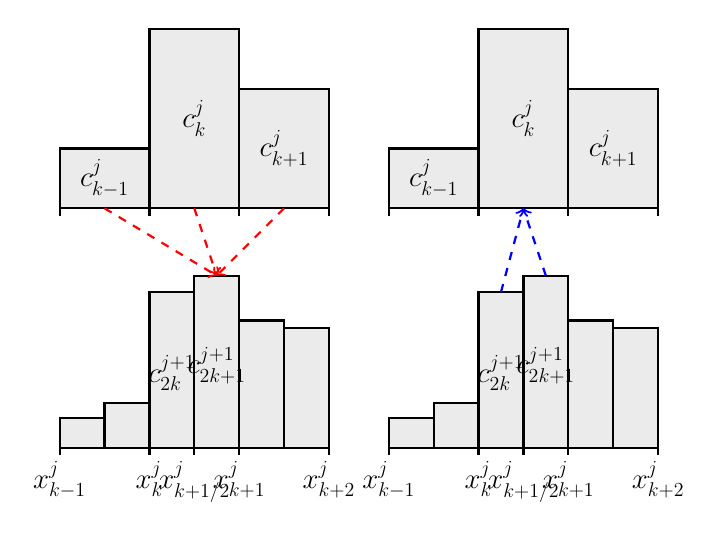
\begin{tikzpicture}[thick,scale=0.38, every node/.style={scale=0.6}]

        % variables
        \def\x{-8.0}
        \def\y{0.0}
        \def\yl{-8.0}

        % draw coarse level rectangles
        \draw [fill=mygray] (\x,0) rectangle (\x+3,2);
        \draw [fill=mygray] (\x+3,0) rectangle (\x+6,6);
        \draw [fill=mygray] (\x+6,0) rectangle (\x+9,4);

        % coarse level symbols
        \node at (\x+1.5,1) {\LARGE $c^{j}_{k-1}$};
        \node at (\x+4.5,3) {\LARGE $c^{j}_{k}$};
        \node at (\x+7.5,2) {\LARGE $c^{j}_{k+1}$};

        % coarse level axis
        \draw (\x,0) -- (\x,-0.25);
        \draw (\x+3,0) -- (\x+3,-0.25);
        \draw (\x+6,0) -- (\x+6,-0.25);
        \draw (\x+9,0) -- (\x+9,-0.25);

        % fine level rectangles
        \draw [fill=mygray] (\x,\yl) rectangle (\x+1.5,\yl+1);
        \draw [fill=mygray] (\x+1.5,\yl) rectangle (\x+3,\yl+1.5);
        \draw [fill=mygray] (\x+3,\yl) rectangle (\x+4.5,\yl+5.2);
        \draw [fill=mygray] (\x+4.5,\yl) rectangle (\x+6,\yl+5.75);
        \draw [fill=mygray] (\x+6,\yl) rectangle (\x+7.5,\yl+4.25);
        \draw [fill=mygray] (\x+7.5,\yl) rectangle (\x+9,\yl+4.0);

        % fine level symbols
        \node at (\x+3.75,\yl+2.5) {\LARGE $c^{j+1}_{2k}$};
        \node at (\x+5.25,\yl+2.75) {\LARGE $c^{j+1}_{2k+1}$};

        % fine level axis
	    \draw (\x,\yl) -- (\x,\yl-0.25);
        \draw (\x+3,\yl) -- (\x+3,\yl-0.25);
        \draw (\x+4.5,\yl) -- (\x+4.5,\yl-0.25);
        \draw (\x+6,\yl) -- (\x+6,\yl-0.25);
	    \draw (\x+9,\yl) -- (\x+9,\yl-0.25);

        % arrows
        \draw[red,dashed,->] (\x+1.5,\y) -- (\x+5.25,\y-2.25);
        \draw[red,dashed,->] (\x+4.5,\y) -- (\x+5.25,\y-2.25);
        \draw[red,dashed,->] (\x+7.5,\y) -- (\x+5.25,\y-2.25);

        % tick text
        \node[below] at (\x,\yl-0.25) {\LARGE $x^{j}_{k-1}$};
        \node[below] at (\x+3,\yl-0.25) {\LARGE $x^{j}_{k}$};
        \node[below] at (\x+4.5,\yl-0.25) {\LARGE $x^{j}_{k+1/2}$};
        \node[below] at (\x+6,\yl-0.25) {\LARGE $x^{j}_{k+1}$};
        \node[below] at (\x+9,\yl-0.25) {\LARGE $x^{j}_{k+2}$};

        %----

        % variables
        \def\x{3.0}
        \def\y{0.0}
        \def\yl{-8.0}

        % draw coarse level rectangles
        \draw [fill=mygray] (\x,0) rectangle (\x+3,2);
        \draw [fill=mygray] (\x+3,0) rectangle (\x+6,6);
        \draw [fill=mygray] (\x+6,0) rectangle (\x+9,4);

        % coarse level symbols
        \node at (\x+1.5,1) {\LARGE $c^{j}_{k-1}$};
        \node at (\x+4.5,3) {\LARGE $c^{j}_{k}$};
        \node at (\x+7.5,2) {\LARGE $c^{j}_{k+1}$};

        % coarse level axis
        \draw (\x,0) -- (\x,-0.25);
        \draw (\x+3,0) -- (\x+3,-0.25);
        \draw (\x+6,0) -- (\x+6,-0.25);
        \draw (\x+9,0) -- (\x+9,-0.25);

        % fine level rectangles
        \draw [fill=mygray] (\x,\yl) rectangle (\x+1.5,\yl+1);
        \draw [fill=mygray] (\x+1.5,\yl) rectangle (\x+3,\yl+1.5);
        \draw [fill=mygray] (\x+3,\yl) rectangle (\x+4.5,\yl+5.2);
        \draw [fill=mygray] (\x+4.5,\yl) rectangle (\x+6,\yl+5.75);
        \draw [fill=mygray] (\x+6,\yl) rectangle (\x+7.5,\yl+4.25);
        \draw [fill=mygray] (\x+7.5,\yl) rectangle (\x+9,\yl+4.0);

        % fine level symbols
        \node at (\x+3.75,\yl+2.5) {\LARGE $c^{j+1}_{2k}$};
        \node at (\x+5.25,\yl+2.75) {\LARGE $c^{j+1}_{2k+1}$};

        % fine level axis
	    \draw (\x,\yl) -- (\x,\yl-0.25);
        \draw (\x+3,\yl) -- (\x+3,\yl-0.25);
        \draw (\x+4.5,\yl) -- (\x+4.5,\yl-0.25);
        \draw (\x+6,\yl) -- (\x+6,\yl-0.25);
	    \draw (\x+9,\yl) -- (\x+9,\yl-0.25);

        % arrows
        \draw[blue,dashed,->] (\x+5.25,\y-2.25) -- (\x+4.5,\y);
        \draw[blue,dashed,->] (\x+3.75,\y-2.8) -- (\x+4.5,\y);

        % tick text
        \node[below] at (\x,\yl-0.25) {\LARGE $x^{j}_{k-1}$};
        \node[below] at (\x+3,\yl-0.25) {\LARGE $x^{j}_{k}$};
        \node[below] at (\x+4.5,\yl-0.25) {\LARGE $x^{j}_{k+1/2}$};
        \node[below] at (\x+6,\yl-0.25) {\LARGE $x^{j}_{k+1}$};
        \node[below] at (\x+9,\yl-0.25) {\LARGE $x^{j}_{k+2}$};


    \end{tikzpicture}
    \caption{Left: quadratic prediction from coarse-scale $j$
        to fine-scale $j+1$, given cell-averages $\mathbf{c}^{j}$.
        Right: Fine-scale cell averages are coarsened.}

\end{figure}
\end{frame}

\section{Multiresolution Code}

\begin{frame}{Multiresolution Code - Examples}
	\begin{figure}
		\center
		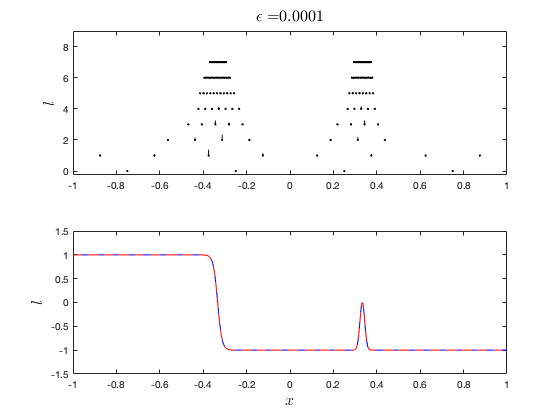
\includegraphics[scale=0.5]{plots/spike-med.png}
		\caption{Better approximation (smaller threshold value).}
	\end{figure}
\end{frame}

\section{Multiresolution Finite Volume Scheme}

\begin{frame}{Multiresolution Scheme on AMR Patches}
	\begin{figure}
		\center
		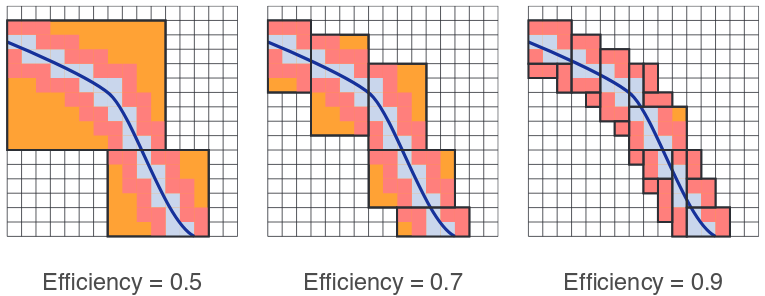
\includegraphics[scale=0.5]{plots/patch-efficiency.png}
		\caption{Increasing patch 'efficiency.'}
	\end{figure}
\end{frame}

\begin{frame}{Multiresolution Scheme on AMR Patches}
      The steps of the scheme for one patch are
      \begin{enumerate}
        \item take given (finest level) data on patch, and coarsen it to desired coarsest level $L$
        \item compute the forward wavelet transform to obtain $\left\{ \mathbf{d}^{l}\right\}_{l=L}^{l=1}$
        \item on coarsest level $L$, compute the residuals $\left\{ R_{j}^{L} \right\}_{j=0}^{N_{L}}$
        \item loop through one finer level at a time, and according to detail coefficients,
              either interpolate or calculate remaining fluxes
      \end{enumerate}
\end{frame}

\begin{frame}{Multiresolution Scheme on AMR Patches}
  The original (fine) data is coarsened by
      \begin{equation*}
        w_{j}^{l} = \frac{1}{2} \left( w_{2j}^{l-1} + w_{2j+1}^{l-1} \right)
      \end{equation*}
      Then the residual $R_{j}^{l}$ may be interpolated in smooth regions as
      \begin{align*}
        R^{l-1}_{2j+1} & = R^{l}_{j} - \frac{1}{8} \left( R^{l}_{j-1} - R^{l}_{j+1} \right) \\
        R^{l-1}_{2j} & = 2 R^{l}_{j} - R^{l-1}_{2j+1}
      \end{align*}
\end{frame}

\begin{frame}[fragile]{Progress in FLASH Implementation}
  \begin{itemize}
    \setlength\itemsep{1em}
    \item created a new folder \texttt{source/flashUtilities/Wavelet/}
    \item writing a program \texttt{Wavelet\_computeTransform.F90} which will be run 
          in \texttt{Grid\_computeUserVars.F90}
  \end{itemize}
  \begin{verbatim}
    function imap( l, i, j, k, nx, ny, nz ) result(x)
      integer, intent(in) :: nx(:), ny(:), nz(:)
      integer, intent(in) :: l, i, j, k
      integer             :: x

      ! compute the map
      x = l + nx * ( i + ny * ( j + nz * k ) )

    end function imap
  \end{verbatim}
\end{frame}


\end{document}
